\section{定积分的分部积分法}
\begin{theorem}\label{theorem:定积分.定积分的分部积分法}
%@see: 《高等数学(第六版 上册)》 P251
%@see: 《数学分析(第二版 上册)》(陈纪修) P300 定理7.3.3
若函数\(u,v \in C[a,b] \cap D(a,b)\),
则\begin{equation}
	\int_a^b u(x) v'(x) \dd{x}
	= \eval{[u(x) v(x)]}_a^b
	- \int_a^b v(x) u'(x) \dd{x},
\end{equation}
或\begin{equation}
	\int_a^b u(x) \dd{[v(x)]}
	= \eval{[u(x) v(x)]}_a^b
	- \int_a^b v(x) \dd{[u(x)]}.
\end{equation}
\end{theorem}
公式表明原函数已经积出的部分可以先用上、下限代入.

\begin{example}
%@see: 《高等数学(第六版 上册)》 P251 例10
计算\(\int_0^{\frac12} \arcsin x \dd{x}\).
\begin{solution}
直接计算得\begin{align*}
	\int_0^{\frac12} \arcsin x \dd{x}
	&= \eval{(x \arcsin x)}_0^{\frac12}
		- \int_0^{\frac12} \frac{x}{\sqrt{1-x^2}} \dd{x} \\
	&= \frac12 \cdot \frac\pi6 + \eval{\sqrt{1-x^2}}_0^{\frac12} \\
	&= \frac\pi{12} + \frac{\sqrt3}2 - 1.
\end{align*}
\end{solution}
\end{example}

\begin{example}
%@see: 《高等数学(第六版 上册)》 P251 例11
计算\(\int_0^1 e^{\sqrt{x}} \dd{x}\).
\begin{solution}
先用换元法.
令\(\sqrt{x}=t\),
则\(x=t^2\),
\(\dd{x} = 2t\dd{t}\),
那么\[
	\int_0^1 e^{\sqrt{x}} \dd{x}
	= 2 \int_0^1 t \dd(e^t)
	= 2 (t e^t)_0^1 - 2 \int_0^1 e^t \dd{t}
	= 2.
\]
\end{solution}
\end{example}

\begin{example}
计算\(\int_0^1 \frac{\arctan x}{1+x} \dd{x}\).
\begin{solution}
首先有\[
	\int_0^1 \frac{\arctan x}{1+x} \dd{x}
	= \eval{\left[\ln(1+x) \arctan x\right]}_0^1
	- \int_0^1 \frac{\ln(1+x)}{1+x^2} \dd{x},
\]
其中\[
	\eval{\left[\ln(1+x) \arctan x\right]}_0^1
	= \ln2 \cdot \frac\pi4 - 0
	= \frac\pi4 \ln2,
\]
而\begin{align*}
	\int_0^1 \frac{\ln(1+x)}{1+x^2} \dd{x}
	&\xlongequal{x=\tan t}
	\int_0^{\pi/4} \frac{\ln(1+\tan t)}{1+\tan^2t} \cdot \sec^2t \dd{t} \\
	&= \int_0^{\pi/4} \ln(1+\tan t) \dd{t} \\
	&= \int_0^{\pi/4} \ln\left[1+\tan(\frac\pi4-t)\right] \dd{t}
		\tag{\cref{theorem:定积分.区间再现}} \\
	&= \int_0^{\pi/4} \ln\left[1+\frac{\tan(\pi/4)-\tan t}{1+\tan(\pi/4) \tan t}\right] \dd{t}
		\tag{\hyperref[equation:函数.三角函数.和积互化公式3]{和积互化公式}} \\
	&= \int_0^{\pi/4} \ln\frac2{1+\tan t} \dd{x} \\
	&= \int_0^{\pi/4} [\ln2 - \ln(1+\tan t)] \dd{x}
		\tag{\hyperref[equation:函数.对数的基本运算法则2]{对数运算法则}} \\
	&= \int_0^{\pi/4} \ln2 \dd{x} - \int_0^{\pi/4} \ln(1+\tan t) \dd{t},
		\tag{\hyperref[theorem:定积分.定积分性质1]{定积分的性质}}
\end{align*}
从而\[
	\int_0^1 \frac{\ln(1+x)}{1+x^2} \dd{x}
	= \int_0^{\pi/4} \ln(1+\tan t) \dd{t}
	= \frac12 \int_0^{\pi/4} \ln2 \dd{x}
	= \frac\pi8 \ln2.
\]
于是\(\int_0^1 \frac{\arctan x}{1+x} \dd{x}
= \frac\pi4 \ln2 - \frac\pi8 \ln2
= \frac\pi8 \ln2\).
\end{solution}
%TODO 据说还有一种换元方法是令\(t = \frac{1-x}{1+x}\),值得一试.
\end{example}

多次运用分部积分公式可以进一步得到以下结果:
\begin{corollary}
设函数\(u,v \in C^{n+1}[a,b]\),
则\[
	\int_a^b u(x) v^{(n+1)}(x) \dd{x}
	= \eval{\left[
		\sum_{k=0}^n (-1)^k u^{(k)}(x) v^{(n-k)}(x)
	\right]}_a^b
	+ (-1)^{n+1} \int_a^b u^{(n+1)}(x) v(x) \dd{x}
\]对\(n=1,2,\dotsc\)均成立.
\end{corollary}

\begin{theorem}\label{theorem:定积分.带有积分余项的泰勒中值定理}
%@see: 《数学分析教程(第3版 上册)》(史济怀) P257 定理6.4.1(Taylor公式的积分余项)
设函数\(f\)在\((a,b)\)上有直到\(n+1\)阶连续导函数,
那么对任意\(x_0\in(a,b)\),
有\begin{equation*}
%\cref{equation:微分中值定理.泰勒公式1}
	f(x) = p_n(x) + R_n(x),
\end{equation*}
其中\begin{gather}
%\cref{equation:微分中值定理.泰勒公式.多项式1}
	p_n(x) = \sum_{k=0}^n \frac{f^{(k)}(x_0)}{k!} (x-x_0)^k, \\
%\cref{equation:微分中值定理.泰勒公式.余项0}
	R_n(x) = \frac1{n!} \int_{x_0}^x (x-t)^n f^{(n+1)}(t) \dd{t}
	\quad(a<x<b).
\end{gather}
%TODO proof
\end{theorem}
\begin{remark}
与\cref{theorem:微分中值定理.泰勒中值定理} 相比,
\cref{theorem:定积分.带有积分余项的泰勒中值定理} 要求的条件稍强,
不仅要求\(f^{(n+1)}\)存在,而且要求它连续.
\end{remark}

\section{正交函数列}
\begin{definition}
%@see: 《数学分析(第二版 上册)》(陈纪修) P300 定义7.3.1
设\(\{g_n\}_{n\geq0}\)是定义在\([a,b]\)上的一列函数.
若对任意\(m,n\in\mathbb{N}\),
函数\(g_m\)和\(g_n\)都在\([a,b]\)上黎曼可积,
且有\[
	\int_a^b g_m(x) g_n(x) \dd{x} = \left\{ \begin{array}{ll}
		0, & m \neq n, \\
		\int_a^b g_n^2(x) \dd{x}, & m = n,
	\end{array} \right.
\]
则称\(\{g_n\}_{n\geq0}\)是“区间\([a,b]\)上的\DefineConcept{正交函数列}”.

特别地,当\(g_n\)是\(n\)次多项式时,
称\(\{g_n\}_{n\geq0}\)是“区间\([a,b]\)上的\DefineConcept{正交多项式函数列}”.
\end{definition}

\begin{example}
%@see: 《数学分析(第二版 上册)》(陈纪修) P301 例7.3.7
证明:拉格朗日多项式\[
	p_n(x) = \frac1{2^n n!} \dv[n]{x} (x^2-1)^n
	\quad(n=0,1,2,\dotsc)
\]组成的函数列\(\{p_n\}_{n\geq0}\)是\([-1,1]\)上的正交多项式函数列.
\begin{proof}
不妨设\(n \geq m\).
记\begin{align*}
	I(m,n) &\defeq m! ~ n! ~ 2^m ~ 2^n \int_{-1}^1 p_m(x) p_n(x) \dd{x} \\
	&= \int_{-1}^1 \dv[m]{x} (x^2-1)^m \cdot \dv[n]{x} (x^2-1)^n \dd{x}.
\end{align*}
只要我们把\(\dv[m]{x} (x^2-1)^m\)看作\(u(x)\),
把\(\dv[n]{x} (x^2-1)^n\)看作\(v'(x)\),
那么利用分部积分法可得\begin{align*}
	I(m,n) = \dv[m]{x} (x^2-1)^m
		\cdot \eval{\dv[n-1]{x} (x^2-1)^n}_{-1}^1
		- \int_{-1}^1 \dv[m+1]{x} (x^2-1)^m
			\cdot \dv[n-1]{x} (x^2-1)^n \dd{x}.
\end{align*}
我们知道,函数\[
	\dv[n-k]{x} (x^2-1)^n
	\quad(k=1,2,\dotsc,n-1)
\]中都含有\((x^2-1)\)因子,
因此\[
	\eval{\dv[n-1]{x} (x^2-1)^n}_{x=1}
	= \eval{\dv[n-1]{x} (x^2-1)^n}_{x=-1}
	= 0,
\]
所以\[
	I(m,n) = - \int_{-1}^1 \dv[m+1]{x} (x^2-1)^m
					\cdot \dv[n-1]{x} (x^2-1)^n \dd{x}.
\]
反复执行上述过程,最后得到\[
	I(m,n) = (-1)^n \int_{-1}^1 \left[\dv[m+n]{x} (x^2-1)^m\right] \cdot (x^2-1)^n \dd{x}.
\]

若\(n>m\),则有\(\dv[m+n]{x} (x^2-1)^m = 0\),
因此\(\int_{-1}^1 p_m(x) p_n(x) \dd{x} = 0\).

若\(n=m\),则有\(\dv[m+n]{x} (x^2-1)^m = (2n)!\),
再次利用分部积分法\begin{align*}
	I(m,n) &= (2n)! \int_{-1}^1 (1-x)^n (1+x)^n \dd{x} \\
	&= \frac{(2n)! n}{n+1} \int_{-1}^1 (1-x)^{n-1} (1+x)^{n+1} \dd{x} \\
	&= \frac{(2n)! n(n-1)}{(n+1)(n+2)} \int_{-1}^1 (1-x)^{n-2} (1+x)^{n+2} \dd{x} \\
	&= \dotsb \\
	&= \frac{(2n)! n(n-1)\dotsm1}{(n+1)(n+2)\dotsm(2n)} \int_{-1}^1 (1+x)^{2n} \dd{x} \\
	&= \frac{(n!)^2 2^{2n+1}}{2n+1}.
\end{align*}
于是便有\[
	\int_{-1}^1 p_n^2(x) \dd{x}
	= \frac1{(n!)^2 2^{2n}} I(m,n)
	= \frac2{2n+1}.
	\qedhere
\]
\end{proof}
\end{example}

\begin{example}\label{example:定积分.点火公式}
%@see: 《高等数学(第六版 上册)》 P251 例12
%@see: 《数学分析(第二版 上册)》(陈纪修) P302 例7.3.8
%@see: 《数学分析教程(第3版 上册)》(史济怀) P259 例3
证明:\begin{equation}\label{equation:定积分.点火公式1}
	I_n = \int_0^{\frac{\pi}{2}} \sin^n x \dd{x}
	= \left\{ \def\arraystretch{1.5} \begin{array}{rl}
		\frac{\pi}{2}\frac{(n-1)!!}{n!!},
			& \text{$n$是偶数}, \\
		\frac{(n-1)!!}{n!!},
			& \text{$n$是奇数}.
	\end{array} \right.
\end{equation}
\begin{proof}
由于\begin{align*}
	I_n &= -\int_0^{\frac{\pi}{2}} \sin^{n-1} x \dd(\cos x) \\
	&= \eval{\left[-\cos x \sin^{n-1} x\right]}_0^{\frac\pi2}
		+ (n-1) \int_0^{\frac\pi2} \sin^{n-2} x \cos^2 x \dd{x} \\
	&= (n-1) \int_0^{\frac\pi2} \sin^{n-2} x (1-\sin^2 x) \dd{x} \\
	&= (n-1) I_{n-2} - (n-1) I_n,
	\end{align*}
所以\[
	I_n = \frac{n-1}{n} I_{n-2}.
\]
于是对于\(k=1,2,\dotsc\)成立\begin{gather*}
	I_{2k}
	= \frac{2k-1}{2k} \cdot \frac{2k-3}{2k-2}
	\cdot \dotsm \cdot \frac{5}{6} \cdot \frac{3}{4} \cdot \frac{1}{2} \cdot I_0, \\
	I_{2k+1}
	= \frac{2k}{2k+1} \cdot \frac{2k-2}{2k-1}
		\cdot \dotsm \cdot \frac{6}{7} \cdot \frac{4}{5} \cdot \frac{2}{3} \cdot I_1.
\end{gather*}
而\[
	I_0 = \int_0^{\frac{\pi}{2}} \dd{x} = \frac{\pi}{2},
	\qquad
	I_1 = \int_0^{\frac{\pi}{2}} \sin x \dd{x} = 1,
\]
因此\begin{gather*}
	I_{2k} = \frac{2k-1}{2k} \cdot \frac{2k-3}{2k-2}
	\cdot \dotsm \cdot \frac{5}{6} \cdot \frac{3}{4}
	\cdot \frac{1}{2} \cdot \frac{\pi}{2}, \\
	I_{2k+1} = \frac{2k}{2k+1} \cdot \frac{2k-2}{2k-1}
		\cdot \dotsm \cdot \frac{6}{7} \cdot \frac{4}{5} \cdot \frac{2}{3}.
	\qedhere
\end{gather*}
\end{proof}
\end{example}
\begin{remark}
由\cref{theorem:定积分.正余弦函数的复合的积分1}
可知\begin{equation}\label{equation:定积分.点火公式2}
	\int_0^{\frac\pi2} \sin^n x \dd{x}
	= \int_0^{\frac\pi2} \cos^n x \dd{x}.
\end{equation}
\end{remark}
\begin{remark}
由诱导公式 \labelcref{equation:函数.三角函数.诱导公式5}
可知\(\sin(\pi-x)=\sin x\),
于是正弦函数\(\sin x\)的正整数次幂的图形
都关于直线\(x=\frac\pi2\)对称
(如\cref{figure:定积分.点火公式}),
那么有\[
	\int_0^{\frac\pi2} \sin^n x \dd{x}
	= \int_{\frac\pi2}^\pi \sin^n x \dd{x},
\]
即有\begin{equation}\label{equation:定积分.点火公式3}
	\int_0^\pi \sin^n x \dd{x}
	= 2 \int_0^{\frac\pi2} \sin^n x \dd{x}.
\end{equation}
%\cref{equation:定积分.区间折半}
\begin{figure}[htb]
	\centering
	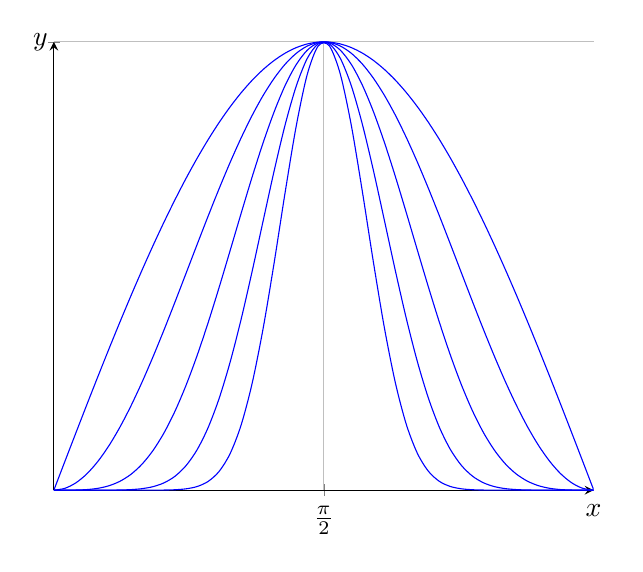
\begin{tikzpicture}
		\begin{axis}[
			xmin=0,xmax=3.14,
			ymin=0,ymax=1,
			grid=both,
			axis lines=middle,
			xlabel=$x$,
			ylabel=$y$,
			x label style={at={(ticklabel* cs:1.00)}, inner sep=5pt, anchor=north},
			y label style={at={(ticklabel* cs:1.00)}, inner sep=2pt, anchor=east},
			ytick={1},
			yticklabels={\relax},
			xtick={1.5708},
			xticklabels={$\frac{\pi}{2}$},
		]
			\addplot[color=blue,samples=50,smooth,domain=0:3.14,variable=\x]{sin(\x r)};
			\addplot[color=blue,samples=50,smooth,domain=0:3.14,variable=\x]{(sin(\x r))^2};
			\addplot[color=blue,samples=50,smooth,domain=0:3.14,variable=\x]{(sin(\x r))^4};
			\addplot[color=blue,samples=50,smooth,domain=0:3.14,variable=\x]{(sin(\x r))^8};
			\addplot[color=blue,samples=50,smooth,domain=0:3.14,variable=\x]{(sin(\x r))^16};
		\end{axis}
	\end{tikzpicture}
	\caption{}
	\label{figure:定积分.点火公式}
\end{figure}

但是由诱导公式 \labelcref{equation:函数.三角函数.诱导公式6}
可知\(\cos(\pi-x)=-\cos x\),
于是只有余弦函数\(\cos x\)的正偶数次幂的图形
都关于直线\(x=\frac\pi2\)对称,
反之,它的正奇数次幂的图形
都关于点\((\frac\pi2,0)\)中心对称,
那么有\begin{equation}\label{equation:定积分.点火公式4}
	\int_0^\pi \cos^n x \dd{x}
	= \left\{ \begin{array}{cl}
		2 \int_0^{\frac\pi2} \sin^n x \dd{x},
		& \text{$n$是偶数}, \\
		0,
		& \text{$n$是奇数}.
	\end{array} \right.
\end{equation}
\end{remark}

下面特别就\cref{equation:定积分.点火公式1} 做一点点展开.
\begin{example}
证明:\begin{equation}
	\lim_{n\to\infty} \int_0^{\frac\pi2} \sin^n x \dd{x} = 0.
\end{equation}
\begin{proof}
因为\(\sin^n\frac{\pi}{2}=1\),
所以对于任意\(n\)总有函数\(\sin^n x\)在点\(\frac{\pi}{2}\)的左邻域取值接近\(1\).
另一方面,对于固定的\(x\)取值,只要\(x<\frac{\pi}{2}\),
则当\(n\)增加时函数值\(\sin^n x\)就很快趋于\(0\).
接下来我们就采用这样的“分而治之”的方法证明
\(\lim_{n\to\infty} \int_0^{\frac\pi2} \sin^n x \dd{x} = 0\).

当\(0<x<\frac{\pi}{2}\)时,\(0<\sin x<1\).
\(\forall\epsilon>0\)(不妨设\(\epsilon<\pi\)).
因为\(\sin x\)在\([0,\pi/2]\)上单调增加且大于零,
故根据\cref{theorem:定积分.定积分性质6},
有\[
	\int_0^{(\pi-\epsilon)/2} \sin^n x \dd{x}
	\leq
	\int_0^{(\pi-\epsilon)/2} \sin^n\frac{\pi-\epsilon}{2} \dd{x}
	\leq
	\frac{\pi}{2} \sin^n\frac{\pi-\epsilon}{2},
\]
因此\[
	0 \leq \int_0^{\frac\pi2} \sin^n x \dd{x}
	= \int_0^{(\pi-\epsilon)/2} \sin^n x \dd{x}
	+ \int_{(\pi-\epsilon)/2}^{\frac\pi2} \sin^n x \dd{x}
	\leq \frac{\pi}{2} \sin^n\frac{\pi-\epsilon}{2} + \frac{\epsilon}{2}.
\]
由\(0<\sin\frac{\pi-\epsilon}{2}<1\),
可见\(\lim_{n\to\infty} \sin^n\frac{\pi-\epsilon}{2} = 0\).
从而对于上述\(\epsilon\),有\[
	(\exists N\in\mathbb{N})
	(\forall n\in\mathbb{N})
	\left[
		\begin{array}{ll}
			n>N
			&\implies
			0<\frac{\pi}{2} \sin^n\frac{\pi-\epsilon}{2}<\frac{\epsilon}{2} \\
			&\implies
			0 \leq \int_0^{\frac\pi2} \sin^n x \dd{s} < \epsilon.
		\end{array}
	\right]
\]
这就证明了\(\lim_{n\to\infty} \int_0^{\frac\pi2} \sin^n x \dd{x} = 0\).
\end{proof}
\end{example}

可以观察到\cref{example:定积分.点火公式} 中,
\(I_{2k}\)和\(I_{2k+1}\)几乎只差一个系数\(\pi/2\).
我们不禁猜想是否可以利用\cref{equation:定积分.点火公式1} 求出圆周率\(\pi\).
\begin{example}[沃利斯公式]
%@see: 《数学分析教程 (第3版 上册)》(史济怀) P309
证明:\begin{equation}\label{equation:定积分.沃利斯公式}
	\lim_{n\to\infty} \frac{1}{2n+1} \left[
		\frac{(2n)!!}{(2n-1)!!}
	\right]^2
	= \frac{\pi}{2}.
\end{equation}
\begin{proof}
因为当\(0<x<\frac{\pi}{2}\)时有\(0<\sin x<1\),
因此对\(\forall n\in\mathbb{N}^*\)就有\[
	\sin^{2n+2} x < \sin^{2n+1} x < \sin^{2n} x.
\]
这样就成立积分不等式\(I_{2n+2} < I_{2n+1} < I_{2n}\),那么\[
	I_{2n+2} = \frac{2n+1}{2n+2} \cdot I_{2n}
	< I_{2n+1} < I_{2n}.
\]
在上式两边同时除以\(I_{2n}\),并取极限,
根据\hyperref[theorem:函数极限.夹逼准则]{夹逼准则}有\[
	\lim_{n\to\infty} \frac{I_{2n+1}}{I_{2n}} = 1
\]
或\[
	\lim_{n\to\infty} \frac{1}{2n+1} \cdot \left[
		\frac{(2n)!!}{(2n-1)!!}
	\right]^2 \cdot \frac{2}{\pi}
	= 1.
	\qedhere
\]
\end{proof}
\end{example}

我们还可以把\hyperref[equation:定积分.沃利斯公式]{沃利斯公式}写成\begin{equation}
%@see: 《数学分析教程 (第3版 上册)》(史济怀) P309 (1)
	\sqrt\pi
	= \lim_{n\to\infty} \frac{(n!)^2 2^{2n}}{(2n)! \sqrt{n}}.
\end{equation}

\begin{example}
计算\[
	I_n = \int_0^\pi x \sin^n x \dd{x}
	\quad(n\in\mathbb{N}^+).
\]
\begin{solution}
直接计算得\begin{align*}
	\int_0^\pi x \sin^n x \dd{x}
	&= \frac\pi2 \int_0^\pi \sin^n x \dd{x}
		\tag{\cref{theorem:定积分.正余弦函数的复合的积分1}} \\
	&= \pi \int_0^{\frac\pi2} \sin^n x \dd{x}.
		\tag{\cref{equation:定积分.点火公式3}}
\end{align*}
\end{solution}
%@Mathematica: Integrate[x Sin[x]^n, {x, 0, Pi}, Assumptions -> {n \[Element] PositiveIntegers}]
\end{example}

\begin{example}
计算:\(\int_0^{2\pi}\left(\int_x^{2\pi}\frac{\sin t}{t}\dd{t}\right)\dd{x}\).
\begin{solution}
这里我们把\(\int_x^{2\pi}\frac{\sin t}{t}\dd{t}\)看成一个整体,
即令\(u = \int_x^{2\pi}\frac{\sin t}{t}\dd{t}\),
那么我们就利用分部积分法,
得到\(\int_0^{2\pi} u \dd{x} = (x u)_0^{2\pi} - \int_0^{2\pi} x \dd{u}\).
按照这个思路,
我们有\begin{align*}
	\int_0^{2\pi}\left(\int_x^{2\pi}\frac{\sin t}{t}\dd{t}\right)\dd{x}
	&= \left(x \int_x^{2\pi}\frac{\sin t}{t}\dd{t}\right)_0^{2\pi}
	- \int_0^{2\pi} x \dd(\int_x^{2\pi}\frac{\sin t}{t}\dd{t}) \\
	&= 0 - \int_0^{2\pi} x \left(-\frac{\sin x}{x}\right) \dd{x} \\
	&= \int_0^{2\pi} \sin x \dd{x} = 0.
\end{align*}
\end{solution}
\end{example}
